\documentclass[12pt, donotrepeattitle, man, floatsintext]{apa6}
\usepackage{amssymb}
\usepackage{graphicx}

\usepackage[outdir=./]{epstopdf}
\usepackage{etoolbox}
\patchcmd{\maketitle}{\newpage}{}{}{}

%\DeclareGraphicsExtensions{.eps}

\usepackage{mathtools}
\usepackage{enumerate}
\usepackage{apacite}
\usepackage{listings}
\usepackage{multirow}
\usepackage{todonotes}
\usepackage{svg}
\usepackage{booktabs}
\usepackage{afterpage}

\newcommand{\den}[2][]{
\(
\left\llbracket\;\text{#2}\;\right\rrbracket^{#1}
\)
}


\newcommand{\KL}[2]{\ensuremath{D_{KL}({#1}\, \| \, {#2})}}
\newcommand{\E}[2]{\ensuremath{\mathbb{E}_{#1}\left [#2 \right]}}

\newenvironment{figurehere}
	{\def\@captype{figure}}
	{}

\setcounter{tocdepth}{2}
\usepackage{lipsum}
%\pagenumbering{gobble}
%\usepackage{apacite}

%\linespread{1}
\usepackage{textcomp}
\usepackage{lingmacros}
\usepackage{setspace}%\doublespacing 

\DeclareGraphicsRule{.tif}{png}{.png}{`convert #1 `dirname #1`/`basename #1 .tif`.png}
\graphicspath{{./figures/}}
 
%\makeatother

\title{Dissertation proposal}
\shorttitle{Dissertation proposal}
\author{Robert Hawkins}
\affiliation{Stanford University} 

%\abstract{}

%\keywords{conventions, pragmatics, semantics, adaptation, learning hierarchical Bayesian models}

%\authornote{This report is based in part on work presented at the 37th Conference of the Cognitive Science Society. The first author is supported by a NSF Graduate Research Fellowship and a Stanford Graduate Fellowship. Correspondence concerning this article should be addressed to Robert X.D. Hawkins, e-mail: rxdh@stanford.edu}

\begin{document}
\thispagestyle{otherpage}

\maketitle
%\tableofcontents

%\section{Introduction}%: Core competencies for adaptation in communication}
Humans spend a great deal of time talking with each other. The relationships we build and the knowledge we share through these interactions is a key ingredient for the success of our species (Henrich, 2015; Tomasello, 2009; Boyd et al, 2011). But how do we manage to understand each other at all? We are not telepathic, so we must coordinate on a system of assigning communicative meaning to the sensory data we produce and perceive (Lewis, 1969). Considerable research efforts have been focused on how such conventional systems could have initially formed and evolved into the highly structured languages of the modern day. Yet we still lack a framework for understanding the challenging but routine coordination problems that remain even for adult speakers of English in full command of their language facility. 

First, no monolithic system of conventions is appropriate for all communicative purposes, and no two speakers of a language share exactly the same lexicon. A wine critic, a therapist, and a neuroscience researcher all need to communicate at a fine level of detail about wildly different topics within their respective communities, and have coordinated on their own idiosyncratic terminology to do so. Lingo, proper nouns, nicknames, slang, inside jokes, metaphors, and other creative uses of neologisms all operate in a regime of uncertainty where the same word or phrase may \emph{a priori} mean something different (or nothing at all) to different partners in different contexts. Second, because our environment is constantly changing, we constantly experience novel entities and events and thoughts and feelings we want to talk about --- complex referents for which we have no pre-existing conventions and real uncertainty about whether a novel compositional utterance will mean to our partner exactly what we intend it to mean. 

In this dissertation, I consider how people manage to communicate so efficiently and accurately under such conditions. I argue that navigating these challenging coordination problems depends critically on the ability to integrate our relatively stable \emph{global conventions} with rapid partner-specific adaptation on \emph{ad hoc} meanings, also known as \emph{local conventions} or \emph{pacts}. The core of this work is an inferential model of convention formation that explains flexible and adaptive language use across extended interaction as a consequence of hierarchical probabilistic learning. Through observing their partner's usage, agents attempt to infer and adopt their partner's underlying lexicon using global conventions as a prior. When both agents independently adopt such a learning strategy, they align to one another, coordinating on and implicitly creating new, shared conventions. 

In brief, the dissertation will proceed as follows (extended abstracts and figures for each chapter are included below; black boxes explain what has already been done and what remains to be done): 
\begin{itemize}
\item Chapter 1 introduces the challenge sketched out above, and lays out the theoretical and empirical landscape that informs my approach.
\item Chapter 2 examines behavior in a rich, natural-language communication task that exposes many of the interesting properties discussed above. In this task, participants must coordinate with one another on a way of repeatedly referring to novel, difficult-to-describe tangram shapes. 
\item Chapter 3 formalizes the theory in a computational model and demonstrates through simulations that it qualitatively captures several core phenomena from earlier chapters.
\item Chapter 4 moves to a simple artificial-language reference game paradigm that deliberately removes participants' dependence on global priors to isolate the dynamics of convention formation. These empirical results demonstrate the effect of communicative context on the conventions that form (i.e. where pragmatics shapes the lexical conventions that emerge from coordination), and also provides a tractable arena for empirically fitting and quantitatively testing our model's predictions.
\item Finally, in Chapter 5, I conclude by discussing the broader implications and future directions of the approach.
\end{itemize}

\section{Chapter 1: Introduction}

Here we lay out the theoretical landscape and empirical evidence focusing on three key aspects of our theoretical approach: (1) the context-sensitive semantic priors that represent our initial uncertainty over what a novel partner is likely to mean by a word, (2) the path-dependence and increasing efficiency of our communicative behavior across even short periods of repeated interaction, and (3) the pattern of generalization from learning local interactions to new contexts and new partners. This review also provides scaffolding for the experimental paradigm used in Chapters 2 and 4 and introduces the phenomena that we capture with our simulations in Chapter 3.

    \vspace{1cm}

\noindent\fbox{%
    \parbox{\textwidth}{%
\textbf{I intend to draw nearly all material in Chapter 1 from revisions on my CADA. Ideally, this introduction would also include a simple meta-analysis of reduction in repeated reference games that has not yet been conducted.}
}
}
\section{Chapter 2: Examining rapid adaptation in a natural-language repeated reference task }

\begin{figure}[t]
\centering
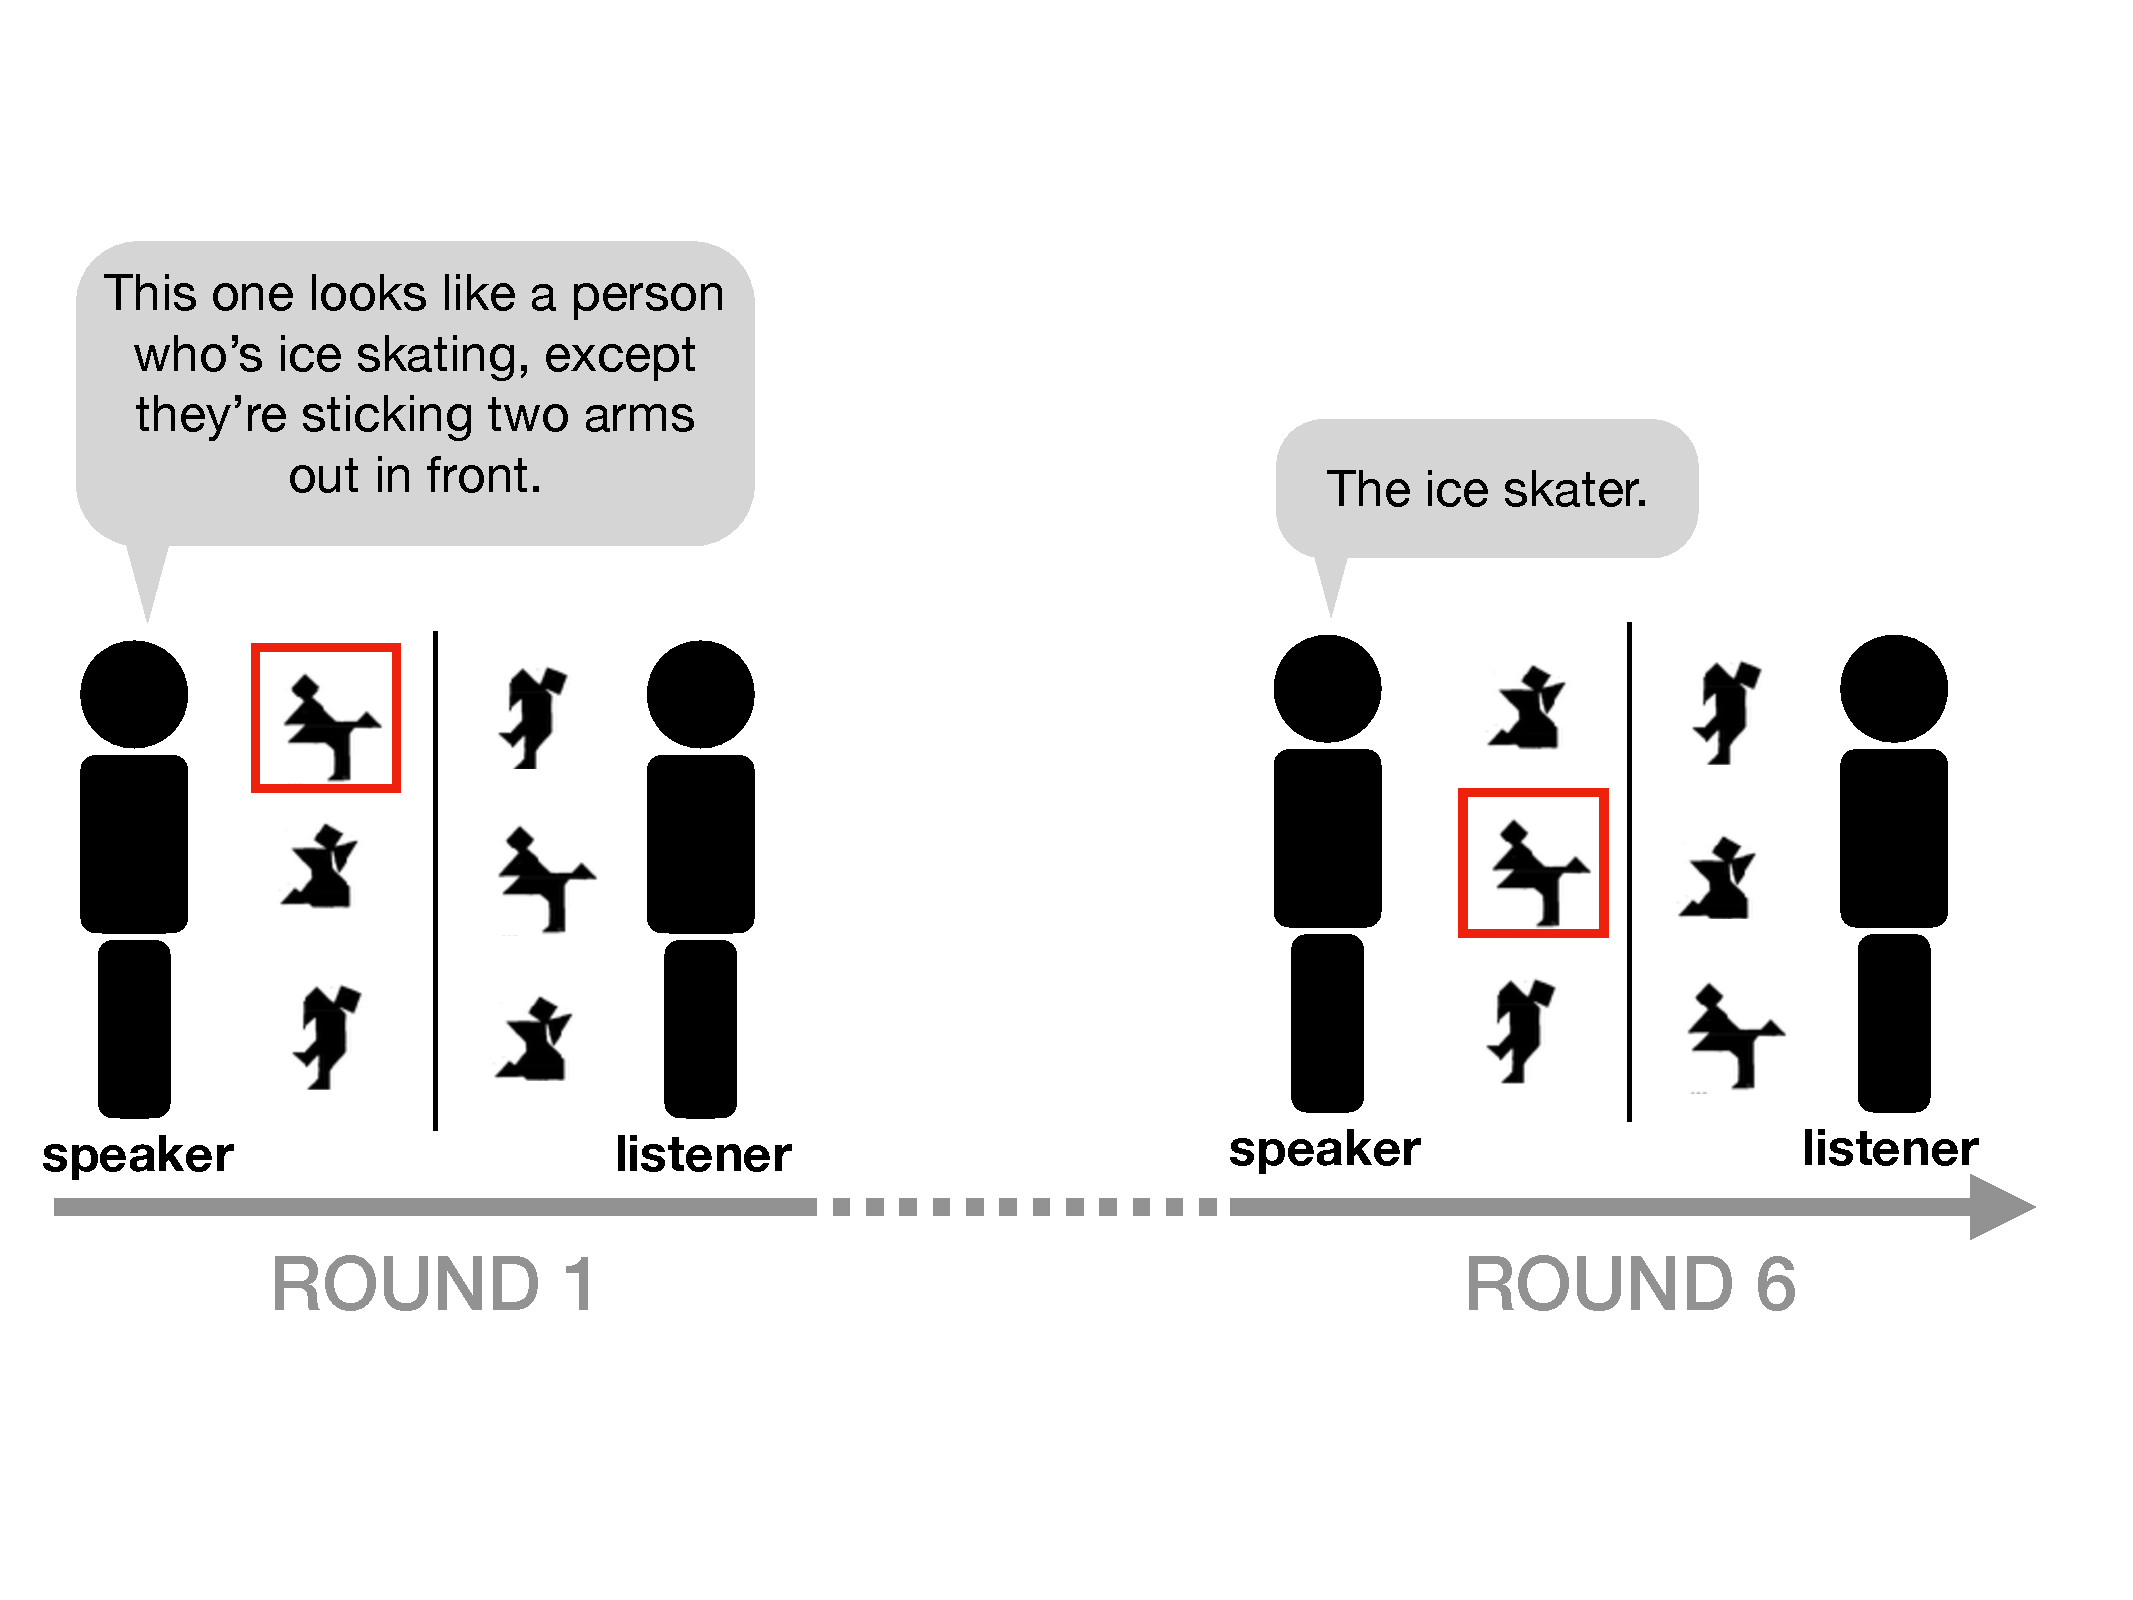
\includegraphics[scale=.45]{task_cropped.pdf}
\caption{Generic setup for repeated reference game task in the lab using stimuli from Wilkes-Gibbs \& Clark (1986); on every round, the speaker refers to each target in some context, and the listener attempts to pick out the intended referent. Both players are free to speak at any time.}
\label{fig:tangramsmethods}
\end{figure}

\begin{figure}[t]
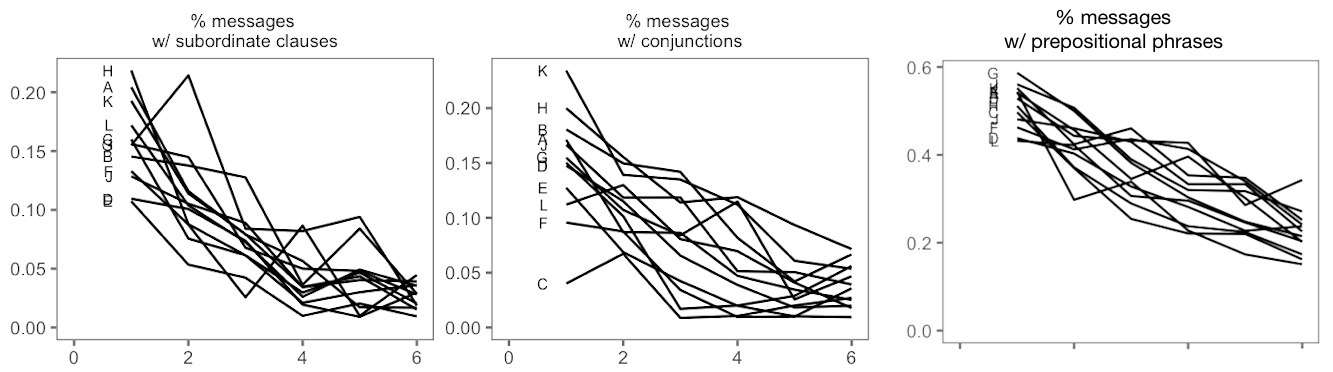
\includegraphics[scale=.35]{tangrams_results.png}
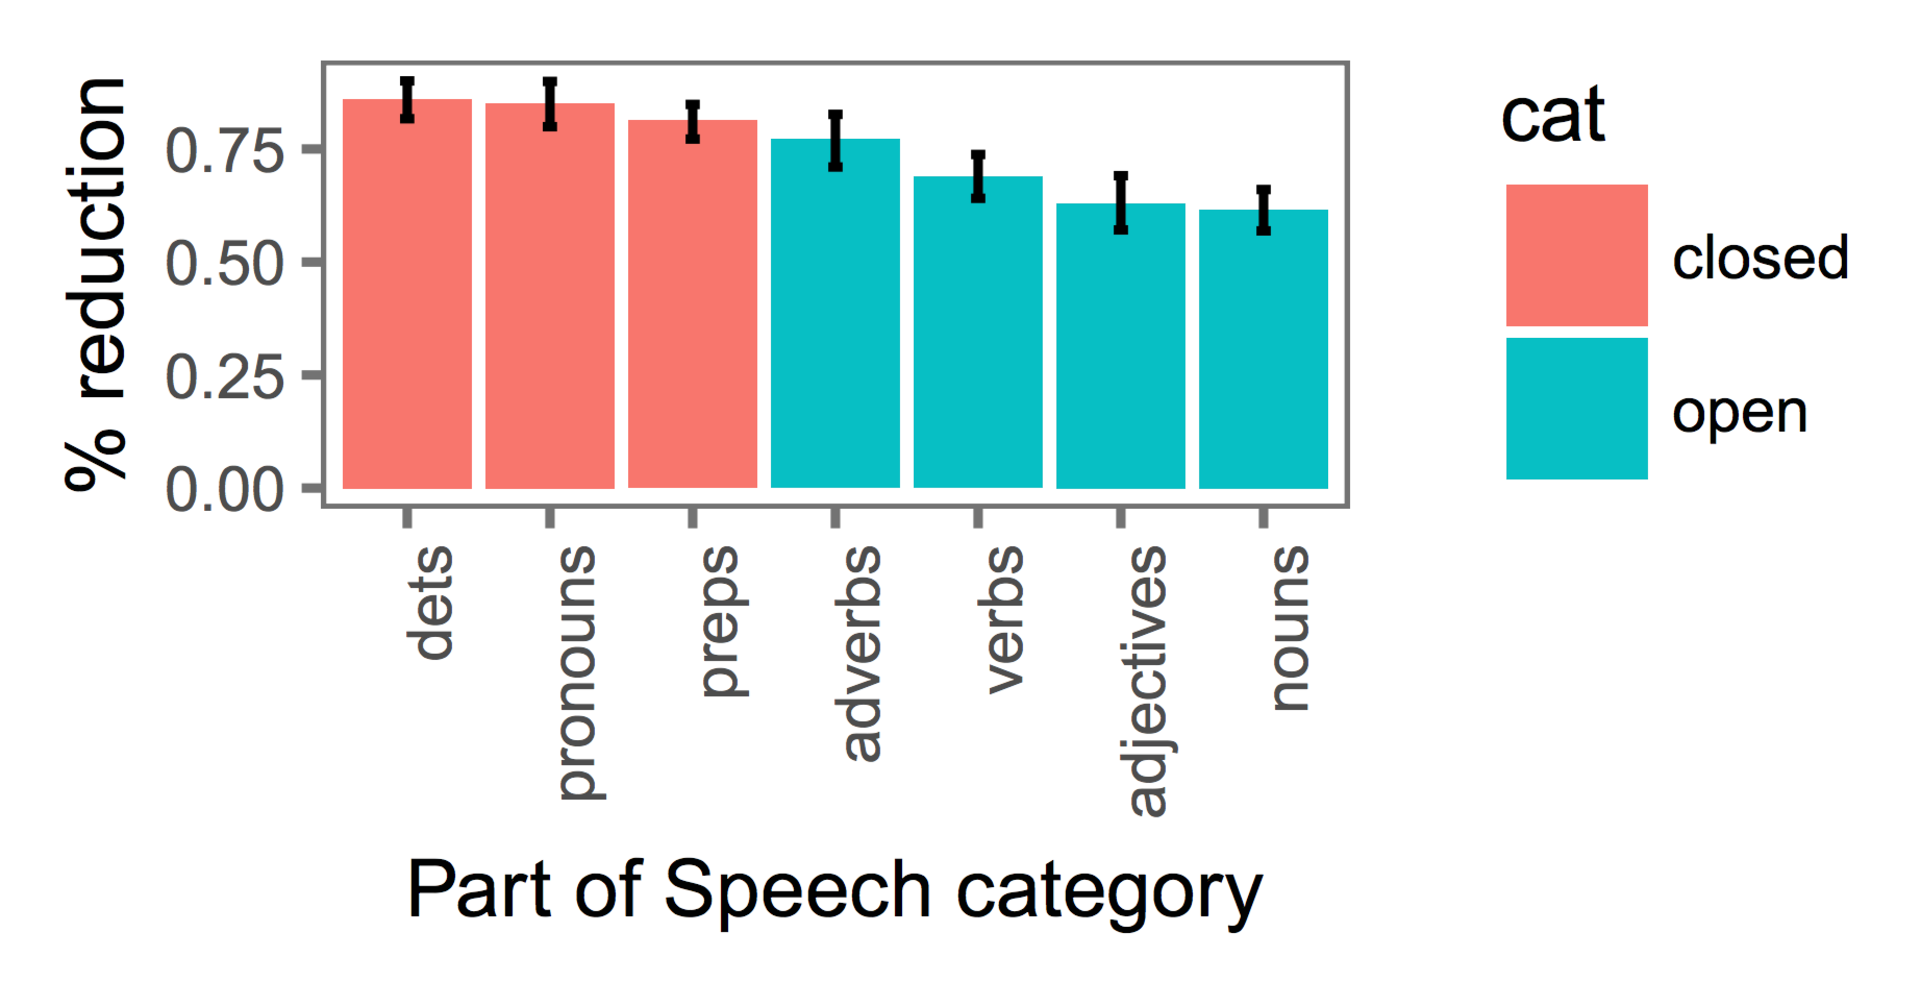
\includegraphics[scale=.25]{pos_fig.pdf}
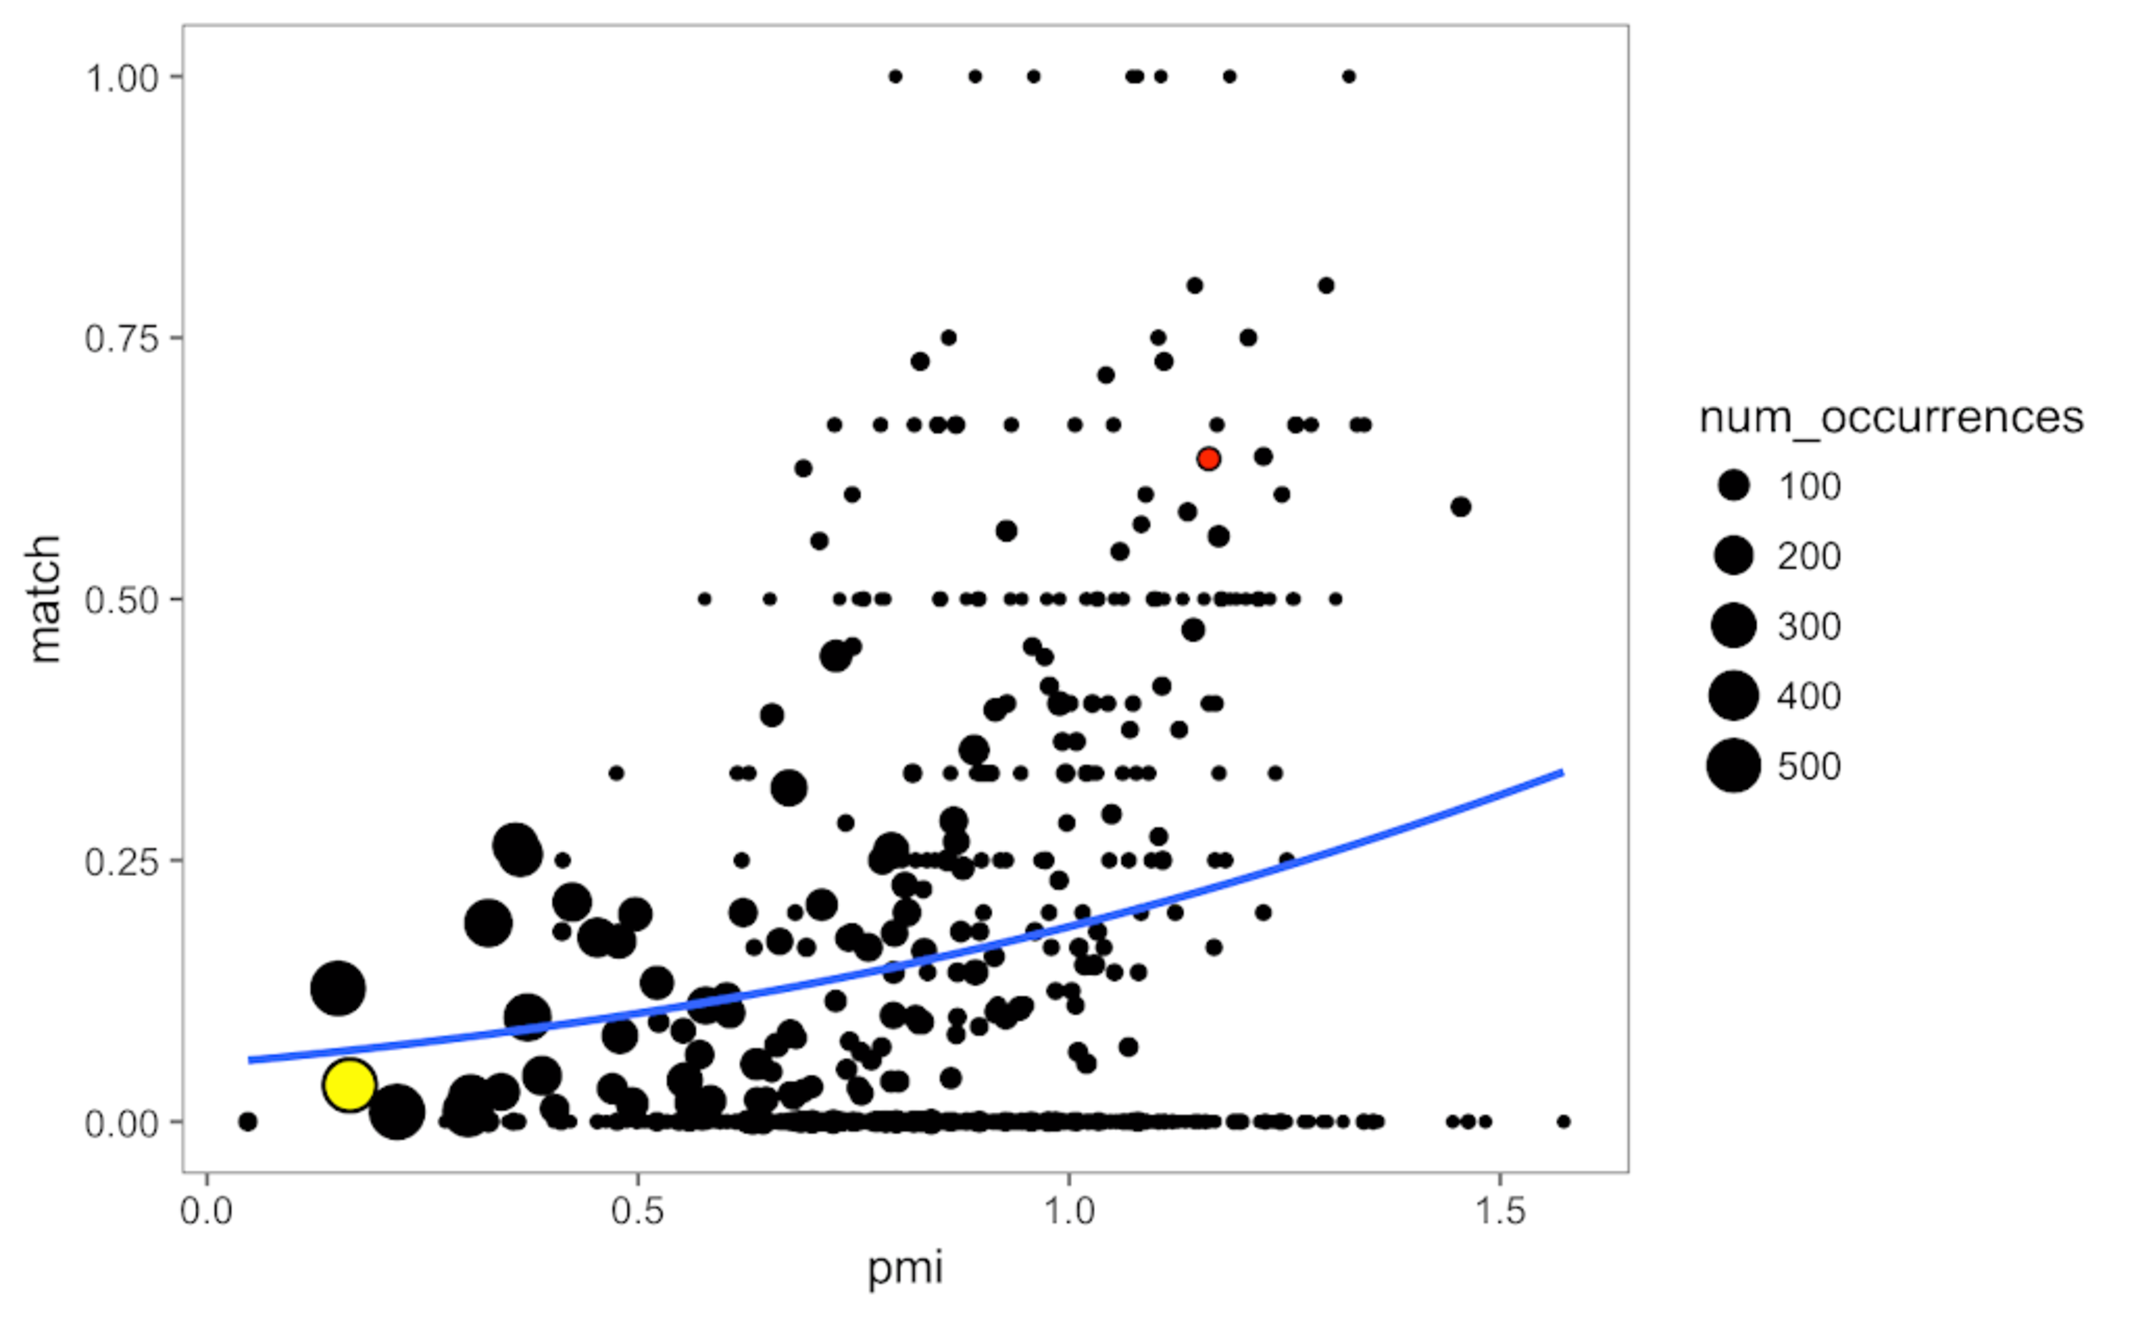
\includegraphics[scale=.25]{pmi.pdf}
\caption{Reduction phenomena reproduced from Hawkins et al, 2017. Clockwise from left: (1) proportion of messages with subordinate clause, broken out by tangram, (2) proportion of messages with conjunction, (3) proportion of utterances containing prepositional phrase, (4) point-wise mutual information on first repetition predicts the likelihood of that word appearing in the final repetition (5) Reduction rates for different parts of speech. Error bars are bootstrapped 95\% CIs}
\label{fig:tangramsresults}
\end{figure}

In a seminal study by Krauss \& Weinheimer (1964), pairs of participants played a cooperative language game where they were presented with arrays of ambiguous shapes in randomized orders. The players were assigned the roles of director and matcher and allowed to talk freely. The matcher's goal was to rearrange their shapes to match the director's board, and the director's goal was to communicate useful descriptions. Over multiple rounds, descriptions were dramatically shortened: an early description like `upside-down martini glass in a wire stand,' became simply `martini' by the end. Later studies (e.g. Clark \& Wilkes-Gibbs, 1986) refined this paradigm, using larger arrays of tangram-like figures (see Fig. 1) and emphasizing the intricate back-and-forth process through which speakers and listeners negotiate over references.

The referring expressions generated by participants across these games reveals a number of rich qualitative phenomena about adaptation in communication. We conduct a large-scale replication of the matching task used by Clark \& Wilkes-Gibbs (1986) as well as a reference game variant with the same stimuli that allows us to track the change in referring expressions over time at a tangram-by-tangram level. We use modern natural language processing techniques to analyze the lexical and syntactic features of utterances and show (1) that the lexical pacts participants form are arbitrary and stable, and (2) that participants are reducing their referring expressions in a systematic and path-dependent manner to preserve distinctive information (see Fig. \ref{fig:tangramsresults}).

\noindent\fbox{%
    \parbox{\textwidth}{%
\textbf{The material in this chapter first appeared in Hawkins, Frank, and Goodman, 2017; Cogsci. Final samples have already been collected for both experiments, and all results have already been written up. Some amount of polishing and verification of the NLP results remains to be done, as well as constructing stricter baselines for several analyses. The plan is to finish this up, revise upon getting feedback from co-authors, and submit in the Fall quarter. }
}
}
\section{Chapter 3: An inferential theory of convention formation}

We propose a hierarchical Bayesian model of convention formation that formalizes our proposal (see Fig. \ref{fig:modelschematic}): global conventions are learned and generalized over many extended interactions with many different people across a lifetime, and  this shared semantic prototype is the backbone supporting rapid learning for new partners and situations. 

Here, we briefly present a sketch of the modeling approach. We begin by defining a lexicon as a function $$\mathcal{L}_i: (w, o) \rightarrow [0,1]$$ assigning any word-object pair a real-valued meaning in the unit interval. Just as our concept of a dog, built up over many individual experiences across a lifetime, provides stable expectations about the properties of a new instance -- four legs, wagging tail, barking noises -- our accumulated lexical knowledge provides stable communicative expectations. 
This knowledge is represented by a `overhypothesis' or shared lexical representation $\Theta_0$, which parameterizes the prior expectations about any individual partner's lexicon: $P(\mathcal{L}_i | \Theta_0)$. 

\begin{figure}[b]
\centering
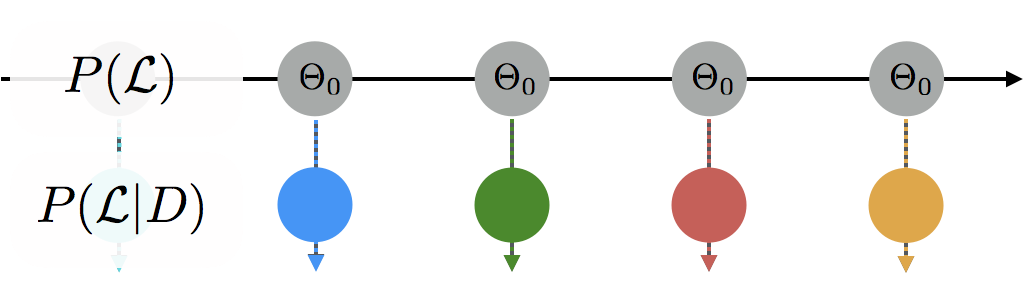
\includegraphics[scale=.4]{model_schematic.png}
\caption{Schematic of our hierarchical model: $\Theta_0$ parameterizes the agent's global beliefs about how their partner uses language, and then through interaction with each partner, they update a partner-specific lexical model based on data $D$ from that interaction.}
\label{fig:modelschematic}
\end{figure}

Now that we have defined a hierarchical likelihood on lexical beliefs, we must say how we \emph{learn} partner-specific models. Our beliefs about a particular partner's lexicon $\mathcal{L}_i$ are formed by integrating our abstract lexical knowledge $\Theta_0$ with particular  observations $D_i$ of that particular individual:
$$%\begin{array}{rcl}
P(\mathcal{L}_i | D_i)  \propto \int_{\Theta_0}P(\mathcal{L}_i | D_i,  \Theta_0) P(\Theta_0 | D_i) 
%                     & = & \mathbb{E}_{\Theta_0}[P(\mathcal{L}_i | \Theta_0, D_i)] 
%\end{array}
$$
where the posteriors in the integral can be computed using Bayes rule:
$$
P(\mathcal{L}_i | D_i, \Theta_0) \propto P(D_i | \mathcal{L}_i, \Theta_0) P(\mathcal{L}_i | \Theta_0)
$$
While this holds when we only have observations from a single speaker, note that our posterior beliefs about $\Theta_0$ are in fact informed by observations from \emph{all} speakers: $D = \bigcup_{i=1}^k D_i$. Finally, to fully specify our model and compute our partner-specific lexical posterior $P(\mathcal{L}_i |D_i, \Theta_0)$, we must link our beliefs about a partner's lexica to their actual behavior with a likelihood function $P(D_i | \mathcal{L}_i, \Theta_0)$. This is naturally supplied by the Rational Speech Act framework: we assume speakers produce utterances that are parsimonious yet informative in context with respect to their lexicon, and listeners interpret utterances by inverting a speaker model. Because we expect our partner to use language rationally given some lexicon, the utterance they choose to refer to some object will be probable under some lexica and highly improbable under others. In this way, a particular agent's language use is a cue to their particular lexicon. 

\begin{figure}[t]
\centering
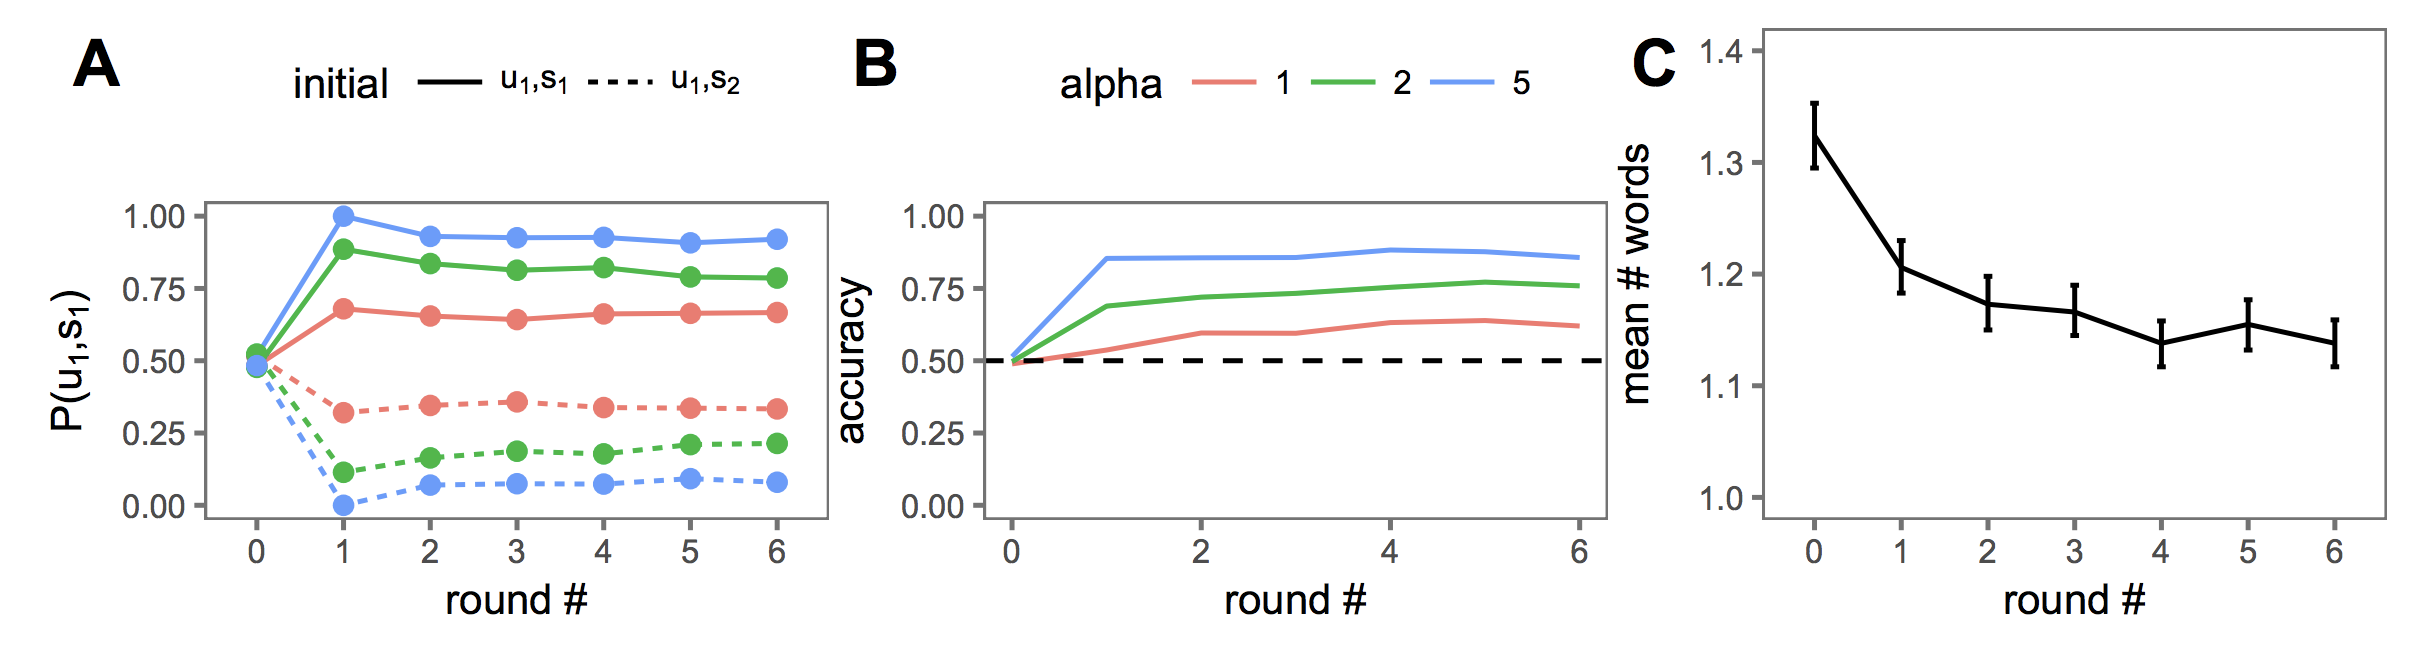
\includegraphics[scale=.36]{model_results.png}
\caption{ (A) Probability of speaker using one of two labels to refer to a state, broken out by initial observation: while players are initially ambivalent between the two labels (arbitrariness), the initial mapping is likely to persist (stability). (B) Accuracy rises as speaker and listener align. (C) When conjunctions are introduced into the grammar, utterances get shorter over time (reduction).}
\label{fig:modelresults}
\end{figure}

First, we show in simulations of a repeated interaction with a single partner that this model successfully allows coordination on arbitrary but path-dependent and stable form-meaning mappings and that a preference for less costly utterances combined with learning gives rise to reduction (see Fig. \ref{fig:modelresults}). Second, we test the generalization properties of our model by manipulating partners and contexts: 
\begin{enumerate}
\item how `sticky' are the pacts formed in one context (i.e. a Dalmatian in the context of other dogs) when the same target is transplanted to a new, less restrictive context (i.e. a Dalmatian in the context of a cat and bear; see Brennen \& Clark, 1996), 
\item to what extent do agents revert to longer utterances after swapping out partners mid-way through a game (see  Wilkes-Gibbs \& Clark, 1992; Metzing \& Brennen, 2003; Yoon \& Brown-Schmidt, 2014), and 
\item how do local, partner-specific expectations generalize to global expectation over repeated interaction with multiple partners in the same community (see Fay et al. 2010).
\end{enumerate}

I also intend to compare this model to other computational approaches to adaptation and convention formation which either fail to account for partner-specific effects or fail to account for patterns of generalization. In particular, the simple RL agents used by Barr (2004), the local priming or consistency heuristics proposed by Garrod \& Pickering (2004) and the heuristic agents from the tradition of Luc Steels (2005), including Centola \& Baronchelli (2015).

\noindent\fbox{%
    \parbox{\textwidth}{%
\textbf{This chapter is based on the initial model simulations reported in Hawkins, Frank, and Goodman, 2017, as well as conceptual work done in the CADA. Because this is an entirely model-based chapter, no additional data must be collected, but a significant amount of work remains to be done to fill this section out over the next year (i.e. all of the context/partner manipulation experiments, lesion experiments testing what components of the model are necessary, and comparisons with other approaches). }
}
}
\vspace{1cm}

\section{Chapter 4: Lexical conventions are shaped by communicative context}

\begin{figure}[b]
\centering
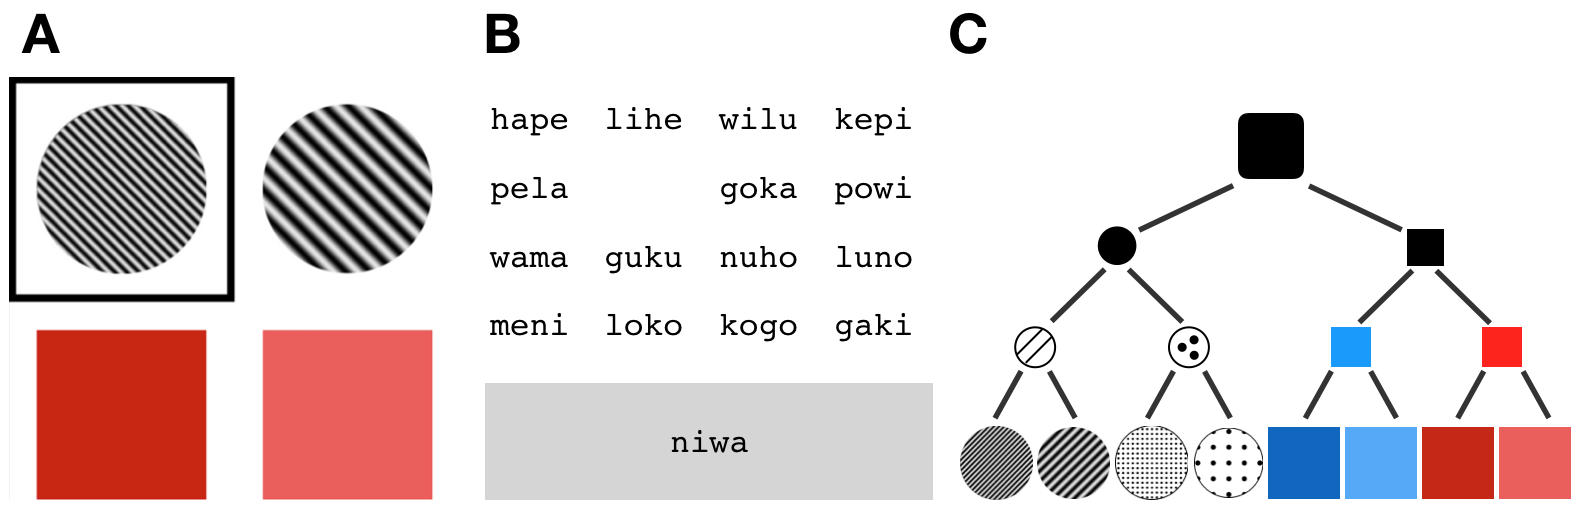
\includegraphics[scale=.5]{fig.png}
\caption{(A) Example of fine context where one of the distractors belongs to the same fine-grained branch of the hierarchy as the target (i.e. another striped circle), so any abstract label would be insufficient to disambiguate them. The target is highlighted for the speaker with a black square. (B) Drag-and-drop chat box interface. (C) Hierarchical organization of stimuli.}
\label{fig:2018task}
\end{figure}

\begin{figure}[t]
\centering
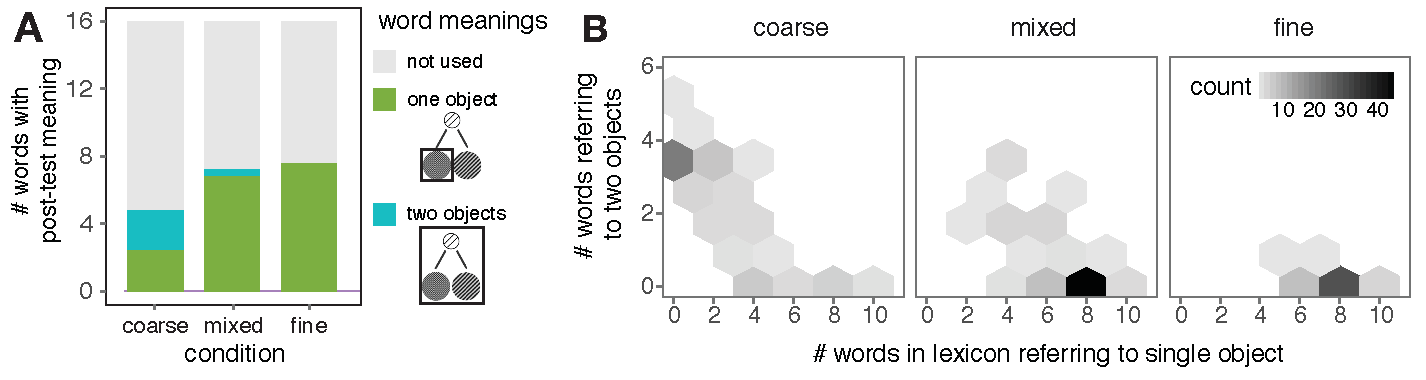
\includegraphics[scale=.7]{resultsFig_v1.pdf}
\caption{ Pragmatic demands of context shape the formation of abstractions. (A) Mean number of words participants reported
with specific meanings (applying to 1 object) or abstract meanings (applying to 2 objects). (B) Diversity of terms within
reported lexica: many participants in the coarse condition reported a mixture of abstract and specific terms.}
\label{fig:modelresults}
\end{figure}

Words exist for referring at many levels of specificity: from the broadest (thing) to the most specific (Fido). What drives the emergence of these taxonomies of reference? Recent computational theories of language evolution suggest that communicative demands of the environment may play a deciding role. Here, we investigate local pragmatic mechanisms of lexical adaptation that may undergird global emergence by manipulating context in a repeated reference game where pairs of participants interactively coordinate on an artificial communication system (see Fig. \ref{fig:2018task}). We hypothesize that pairs should coordinate on conventions for specific names (e.g. Fido) when the context requires frequently making fine distinctions between entities; conversely, they should converge on a more compressed system of conventions for abstract categories (e.g. dog) in coarser contexts, even if a finer mapping would be sufficient. We show differences in the levels of abstraction that emerged in different environments (see Fig. \ref{fig:2018task}) and introduce a statistical approach to probe the dynamics of emergence. Finally, we use these data as a quantitative test for the model we proposed in Chapter 3. 

\vspace{1cm}
\noindent\fbox{%
    \parbox{\textwidth}{%
\textbf{The first experiment in this section is written up in Hawkins, Franke, Smith, \& Goodman, 2018; Cogsci. While this paper included a statistical model inferring lexical meaning over time using RSA, I have not yet attempted to fit the cognitive model from Chapter 3 to these data. To pursue the question of why multiple levels of a conceptual hierarchy are lexicalized, I also intend to run an additional experiment asking participants to refer to a set of targets instead of a singleton, and to test the model in this case as well.
}
    }%
}

%There are \emph{many} potential ways this function could be represented in the mind at the algorithmic level. It could be derived from a store of exemplars, a set of independent prototypes for each word, a neural network embedding words and objects in a vector space, and so on \cite<see>[for a recent review of candidates]{JonesEtAl15_SemanticMemory}.

\section{Chapter 5: Conclusions and future directions}

Language is not some monolithic body of knowledge that we acquire at an early age and deploy mechanically for the rest of our lives. Nor is its evolution a slow, inter-generational drift. It is a means for communication -- a shared interface between minds -- and must therefore adapt over the rapid timescales required by communication. In other words, we are constantly learning language. Not just one language, but an enormous family of related languages, across every repeated interaction with every partner. In this chapter, we discuss directions for future work and broader implications for language acquisition,  neural systems supporting adaptive communication, hierarchical semantic embeddings for human-robot interaction, theories of meaning in philosophy, and the spread of conventions across larger social networks.

\vspace{1cm}
\noindent\fbox{%
    \parbox{\textwidth}{%
\textbf{This section will be compiled from grant and fellowship proposals I'm writing in the upcoming year, as well as text written for ongoing projects}
}
    }%


%\section{\bf Acknowledgments}
%\small
%\noindent RXDH was supported by the Stanford Graduate Fellowship and the National Science Foundation Graduate Research Fellowship under Grant No. DGE-114747.

\small
\singlespacing
\bibliography{cada}
\bibliographystyle{apacite}


\end{document}  
